\documentclass[1p]{elsarticle_modified}
%\bibliographystyle{elsarticle-num}

%\usepackage[colorlinks]{hyperref}
%\usepackage{abbrmath_seonhwa} %\Abb, \Ascr, \Acal ,\Abf, \Afrak
\usepackage{amsfonts}
\usepackage{amssymb}
\usepackage{amsmath}
\usepackage{amsthm}
\usepackage{scalefnt}
\usepackage{amsbsy}
\usepackage{kotex}
\usepackage{caption}
\usepackage{subfig}
\usepackage{color}
\usepackage{graphicx}
\usepackage{xcolor} %% white, black, red, green, blue, cyan, magenta, yellow
\usepackage{float}
\usepackage{setspace}
\usepackage{hyperref}

\usepackage{tikz}
\usetikzlibrary{arrows}

\usepackage{multirow}
\usepackage{array} % fixed length table
\usepackage{hhline}

%%%%%%%%%%%%%%%%%%%%%
\makeatletter
\renewcommand*\env@matrix[1][\arraystretch]{%
	\edef\arraystretch{#1}%
	\hskip -\arraycolsep
	\let\@ifnextchar\new@ifnextchar
	\array{*\c@MaxMatrixCols c}}
\makeatother %https://tex.stackexchange.com/questions/14071/how-can-i-increase-the-line-spacing-in-a-matrix
%%%%%%%%%%%%%%%

\usepackage[normalem]{ulem}

\newcommand{\msout}[1]{\ifmmode\text{\sout{\ensuremath{#1}}}\else\sout{#1}\fi}
%SOURCE: \msout is \stkout macro in https://tex.stackexchange.com/questions/20609/strikeout-in-math-mode

\newcommand{\cancel}[1]{
	\ifmmode
	{\color{red}\msout{#1}}
	\else
	{\color{red}\sout{#1}}
	\fi
}

\newcommand{\add}[1]{
	{\color{blue}\uwave{#1}}
}

\newcommand{\replace}[2]{
	\ifmmode
	{\color{red}\msout{#1}}{\color{blue}\uwave{#2}}
	\else
	{\color{red}\sout{#1}}{\color{blue}\uwave{#2}}
	\fi
}

\newcommand{\Sol}{\mathcal{S}} %segment
\newcommand{\D}{D} %diagram
\newcommand{\A}{\mathcal{A}} %arc


%%%%%%%%%%%%%%%%%%%%%%%%%%%%%5 test

\def\sl{\operatorname{\textup{SL}}(2,\Cbb)}
\def\psl{\operatorname{\textup{PSL}}(2,\Cbb)}
\def\quan{\mkern 1mu \triangleright \mkern 1mu}

\theoremstyle{definition}
\newtheorem{thm}{Theorem}[section]
\newtheorem{prop}[thm]{Proposition}
\newtheorem{lem}[thm]{Lemma}
\newtheorem{ques}[thm]{Question}
\newtheorem{cor}[thm]{Corollary}
\newtheorem{defn}[thm]{Definition}
\newtheorem{exam}[thm]{Example}
\newtheorem{rmk}[thm]{Remark}
\newtheorem{alg}[thm]{Algorithm}

\newcommand{\I}{\sqrt{-1}}
\begin{document}

%\begin{frontmatter}
%
%\title{Boundary parabolic representations of knots up to 8 crossings}
%
%%% Group authors per affiliation:
%\author{Yunhi Cho} 
%\address{Department of Mathematics, University of Seoul, Seoul, Korea}
%\ead{yhcho@uos.ac.kr}
%
%
%\author{Seonhwa Kim} %\fnref{s_kim}}
%\address{Center for Geometry and Physics, Institute for Basic Science, Pohang, 37673, Korea}
%\ead{ryeona17@ibs.re.kr}
%
%\author{Hyuk Kim}
%\address{Department of Mathematical Sciences, Seoul National University, Seoul 08826, Korea}
%\ead{hyukkim@snu.ac.kr}
%
%\author{Seokbeom Yoon}
%\address{Department of Mathematical Sciences, Seoul National University, Seoul, 08826,  Korea}
%\ead{sbyoon15@snu.ac.kr}
%
%\begin{abstract}
%We find all boundary parabolic representation of knots up to 8 crossings.
%
%\end{abstract}
%\begin{keyword}
%    \MSC[2010] 57M25 
%\end{keyword}
%
%\end{frontmatter}

%\linenumbers
%\tableofcontents
%
\newcommand\colored[1]{\textcolor{white}{\rule[-0.35ex]{0.8em}{1.4ex}}\kern-0.8em\color{red} #1}%
%\newcommand\colored[1]{\textcolor{white}{ #1}\kern-2.17ex	\textcolor{white}{ #1}\kern-1.81ex	\textcolor{white}{ #1}\kern-2.15ex\color{red}#1	}

{\Large $\underline{12n_{0875}~(K12n_{0875})}$}

\setlength{\tabcolsep}{10pt}
\renewcommand{\arraystretch}{1.6}
\vspace{1cm}\begin{tabular}{m{100pt}>{\centering\arraybackslash}m{274pt}}
\multirow{5}{120pt}{
	\centering
	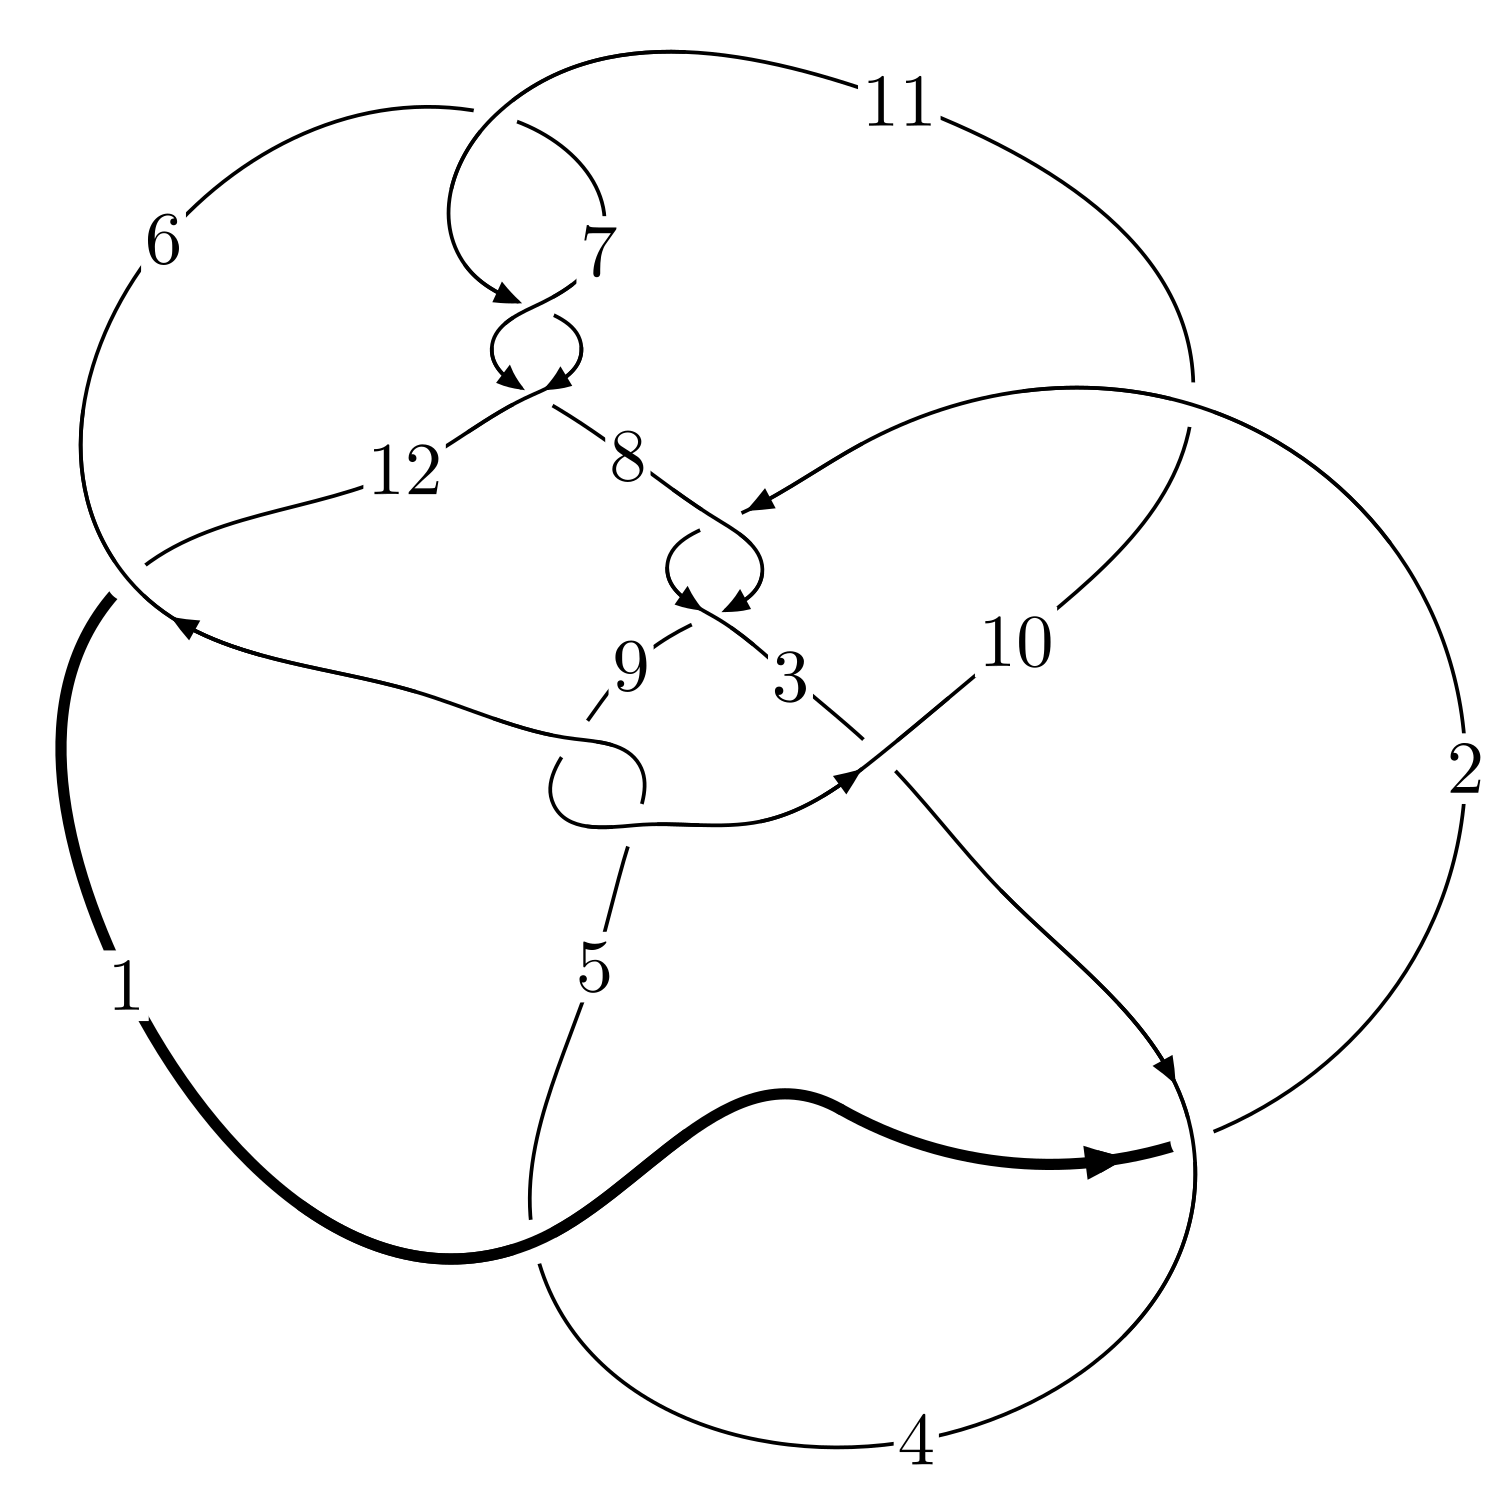
\includegraphics[width=112pt]{../../../GIT/diagram.site/Diagrams/png/2964_12n_0875.png}\\
\ \ \ A knot diagram\footnotemark}&
\allowdisplaybreaks
\textbf{Linearized knot diagam} \\
\cline{2-2}
 &
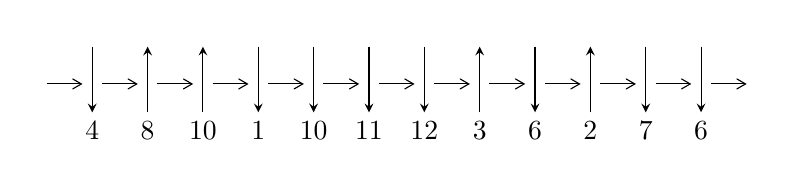
\begin{tikzpicture}[x=20pt, y=17pt]
	% nodes
	\node (C0) at (0, 0) {};
	\node (C1) at (1, 0) {};
	\node (C1U) at (1, +1) {};
	\node (C1D) at (1, -1) {4};

	\node (C2) at (2, 0) {};
	\node (C2U) at (2, +1) {};
	\node (C2D) at (2, -1) {8};

	\node (C3) at (3, 0) {};
	\node (C3U) at (3, +1) {};
	\node (C3D) at (3, -1) {10};

	\node (C4) at (4, 0) {};
	\node (C4U) at (4, +1) {};
	\node (C4D) at (4, -1) {1};

	\node (C5) at (5, 0) {};
	\node (C5U) at (5, +1) {};
	\node (C5D) at (5, -1) {10};

	\node (C6) at (6, 0) {};
	\node (C6U) at (6, +1) {};
	\node (C6D) at (6, -1) {11};

	\node (C7) at (7, 0) {};
	\node (C7U) at (7, +1) {};
	\node (C7D) at (7, -1) {12};

	\node (C8) at (8, 0) {};
	\node (C8U) at (8, +1) {};
	\node (C8D) at (8, -1) {3};

	\node (C9) at (9, 0) {};
	\node (C9U) at (9, +1) {};
	\node (C9D) at (9, -1) {6};

	\node (C10) at (10, 0) {};
	\node (C10U) at (10, +1) {};
	\node (C10D) at (10, -1) {2};

	\node (C11) at (11, 0) {};
	\node (C11U) at (11, +1) {};
	\node (C11D) at (11, -1) {7};

	\node (C12) at (12, 0) {};
	\node (C12U) at (12, +1) {};
	\node (C12D) at (12, -1) {6};
	\node (C13) at (13, 0) {};

	% arrows
	\draw[->,>={angle 60}]
	(C0) edge (C1) (C1) edge (C2) (C2) edge (C3) (C3) edge (C4) (C4) edge (C5) (C5) edge (C6) (C6) edge (C7) (C7) edge (C8) (C8) edge (C9) (C9) edge (C10) (C10) edge (C11) (C11) edge (C12) (C12) edge (C13) ;	\draw[->,>=stealth]
	(C1U) edge (C1D) (C2D) edge (C2U) (C3D) edge (C3U) (C4U) edge (C4D) (C5U) edge (C5D) (C6U) edge (C6D) (C7U) edge (C7D) (C8D) edge (C8U) (C9U) edge (C9D) (C10D) edge (C10U) (C11U) edge (C11D) (C12U) edge (C12D) ;
	\end{tikzpicture} \\
\hhline{~~} \\& 
\textbf{Solving Sequence} \\ \cline{2-2} 
 &
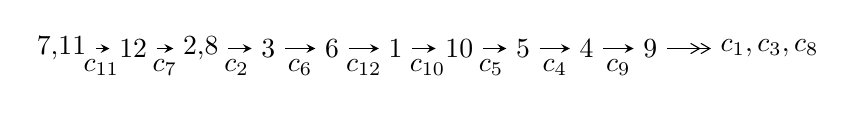
\begin{tikzpicture}[x=23pt, y=7pt]
	% node
	\node (A0) at (-1/8, 0) {7,11};
	\node (A1) at (1, 0) {12};
	\node (A2) at (33/16, 0) {2,8};
	\node (A3) at (25/8, 0) {3};
	\node (A4) at (33/8, 0) {6};
	\node (A5) at (41/8, 0) {1};
	\node (A6) at (49/8, 0) {10};
	\node (A7) at (57/8, 0) {5};
	\node (A8) at (65/8, 0) {4};
	\node (A9) at (73/8, 0) {9};
	\node (C1) at (1/2, -1) {$c_{11}$};
	\node (C2) at (3/2, -1) {$c_{7}$};
	\node (C3) at (21/8, -1) {$c_{2}$};
	\node (C4) at (29/8, -1) {$c_{6}$};
	\node (C5) at (37/8, -1) {$c_{12}$};
	\node (C6) at (45/8, -1) {$c_{10}$};
	\node (C7) at (53/8, -1) {$c_{5}$};
	\node (C8) at (61/8, -1) {$c_{4}$};
	\node (C9) at (69/8, -1) {$c_{9}$};
	\node (A10) at (11, 0) {$c_{1},c_{3},c_{8}$};

	% edge
	\draw[->,>=stealth]	
	(A0) edge (A1) (A1) edge (A2) (A2) edge (A3) (A3) edge (A4) (A4) edge (A5) (A5) edge (A6) (A6) edge (A7) (A7) edge (A8) (A8) edge (A9) ;
	\draw[->>,>={angle 60}]	
	(A9) edge (A10);
\end{tikzpicture} \\ 

\end{tabular} \\

\footnotetext{
The image of knot diagram is generated by the software ``\textbf{Draw programme}" developed by Andrew Bartholomew(\url{http://www.layer8.co.uk/maths/draw/index.htm\#Running-draw}), where we modified some parts for our purpose(\url{https://github.com/CATsTAILs/LinksPainter}).
}\phantom \\ \newline 
\centering \textbf{Ideals for irreducible components\footnotemark of $X_{\text{par}}$} 
 
\begin{align*}
I^u_{1}&=\langle 
-41 u^{26}+353 u^{25}+\cdots+8 b+776,\;-421 u^{26}+3271 u^{25}+\cdots+16 a+5248,\\
\phantom{I^u_{1}}&\phantom{= \langle  }u^{27}-9 u^{26}+\cdots+32 u+16\rangle \\
I^u_{2}&=\langle 
5.05025\times10^{19} a^{7} u^{4}+2.52836\times10^{19} a^{6} u^{4}+\cdots-5.62996\times10^{20} a-3.53454\times10^{20},\\
\phantom{I^u_{2}}&\phantom{= \langle  }a^7 u^4+2 a^6 u^4+\cdots+2 a+8,\;u^5+u^4-2 u^3- u^2+u-1\rangle \\
I^u_{3}&=\langle 
- u^{17}+u^{16}+\cdots+b-1,\;- u^{17}+2 u^{16}+\cdots+a+1,\;u^{18}-10 u^{16}+\cdots+2 u+1\rangle \\
\\
\end{align*}
\raggedright * 3 irreducible components of $\dim_{\mathbb{C}}=0$, with total 85 representations.\\
\footnotetext{All coefficients of polynomials are rational numbers. But the coefficients are sometimes approximated in decimal forms when there is not enough margin.}
\newpage
\renewcommand{\arraystretch}{1}
\centering \section*{I. $I^u_{1}= \langle -41 u^{26}+353 u^{25}+\cdots+8 b+776,\;-421 u^{26}+3271 u^{25}+\cdots+16 a+5248,\;u^{27}-9 u^{26}+\cdots+32 u+16 \rangle$}
\flushleft \textbf{(i) Arc colorings}\\
\begin{tabular}{m{7pt} m{180pt} m{7pt} m{180pt} }
\flushright $a_{7}=$&$\begin{pmatrix}0\\u\end{pmatrix}$ \\
\flushright $a_{11}=$&$\begin{pmatrix}1\\0\end{pmatrix}$ \\
\flushright $a_{12}=$&$\begin{pmatrix}1\\u^2\end{pmatrix}$ \\
\flushright $a_{2}=$&$\begin{pmatrix}\frac{421}{16} u^{26}-\frac{3271}{16} u^{25}+\cdots-900 u-328\\\frac{41}{8} u^{26}-\frac{353}{8} u^{25}+\cdots-287 u-97\end{pmatrix}$ \\
\flushright $a_{8}=$&$\begin{pmatrix}- u\\- u^3+u\end{pmatrix}$ \\
\flushright $a_{3}=$&$\begin{pmatrix}\frac{389}{16} u^{26}-\frac{2911}{16} u^{25}+\cdots-639 u-246\\\frac{185}{8} u^{26}-\frac{1413}{8} u^{25}+\cdots-660 u-251\end{pmatrix}$ \\
\flushright $a_{6}=$&$\begin{pmatrix}u\\u\end{pmatrix}$ \\
\flushright $a_{1}=$&$\begin{pmatrix}- u^4+u^2+1\\- u^4+2 u^2\end{pmatrix}$ \\
\flushright $a_{10}=$&$\begin{pmatrix}-9.50000 u^{26}+71.5000 u^{25}+\cdots+263.500 u+100.500\\-6 u^{26}+\frac{93}{2} u^{25}+\cdots+\frac{393}{2} u+72\end{pmatrix}$ \\
\flushright $a_{5}=$&$\begin{pmatrix}\frac{95}{4} u^{26}-\frac{689}{4} u^{25}+\cdots-\frac{2027}{4} u-204\\\frac{143}{4} u^{26}-267 u^{25}+\cdots-951 u-364\end{pmatrix}$ \\
\flushright $a_{4}=$&$\begin{pmatrix}-34 u^{26}+\frac{997}{4} u^{25}+\cdots+\frac{3177}{4} u+312\\-\frac{61}{4} u^{26}+114 u^{25}+\cdots+409 u+156\end{pmatrix}$ \\
\flushright $a_{9}=$&$\begin{pmatrix}2 u^{26}-\frac{25}{2} u^{25}+\cdots-\frac{1}{2} u-\frac{7}{2}\\\frac{11}{2} u^{26}-\frac{75}{2} u^{25}+\cdots-\frac{135}{2} u-32\end{pmatrix}$\\&\end{tabular}
\flushleft \textbf{(ii) Obstruction class $= -1$}\\~\\
\flushleft \textbf{(iii) Cusp Shapes $= \frac{21}{2} u^{26}-\frac{155}{2} u^{25}+\cdots-328 u-122$}\\~\\
\newpage\renewcommand{\arraystretch}{1}
\flushleft \textbf{(iv) u-Polynomials at the component}\newline \\
\begin{tabular}{m{50pt}|m{274pt}}
Crossings & \hspace{64pt}u-Polynomials at each crossing \\
\hline $$\begin{aligned}c_{1},c_{4}\end{aligned}$$&$\begin{aligned}
&u^{27}-12 u^{26}+\cdots+208 u-32
\end{aligned}$\\
\hline $$\begin{aligned}c_{2},c_{8},c_{10}\end{aligned}$$&$\begin{aligned}
&u^{27}- u^{26}+\cdots- u^2+1
\end{aligned}$\\
\hline $$\begin{aligned}c_{3}\end{aligned}$$&$\begin{aligned}
&u^{27}+14 u^{25}+\cdots+15 u+6
\end{aligned}$\\
\hline $$\begin{aligned}c_{5},c_{9}\end{aligned}$$&$\begin{aligned}
&u^{27}+u^{26}+\cdots+3 u+1
\end{aligned}$\\
\hline $$\begin{aligned}c_{6},c_{7},c_{11}\end{aligned}$$&$\begin{aligned}
&u^{27}-9 u^{26}+\cdots+32 u+16
\end{aligned}$\\
\hline $$\begin{aligned}c_{12}\end{aligned}$$&$\begin{aligned}
&u^{27}+27 u^{26}+\cdots+69984 u+2544
\end{aligned}$\\
\hline
\end{tabular}\\~\\
\newpage\renewcommand{\arraystretch}{1}
\flushleft \textbf{(v) Riley Polynomials at the component}\newline \\
\begin{tabular}{m{50pt}|m{274pt}}
Crossings & \hspace{64pt}Riley Polynomials at each crossing \\
\hline $$\begin{aligned}c_{1},c_{4}\end{aligned}$$&$\begin{aligned}
&y^{27}+12 y^{26}+\cdots+2816 y-1024
\end{aligned}$\\
\hline $$\begin{aligned}c_{2},c_{8},c_{10}\end{aligned}$$&$\begin{aligned}
&y^{27}-11 y^{26}+\cdots+2 y-1
\end{aligned}$\\
\hline $$\begin{aligned}c_{3}\end{aligned}$$&$\begin{aligned}
&y^{27}+28 y^{26}+\cdots-735 y-36
\end{aligned}$\\
\hline $$\begin{aligned}c_{5},c_{9}\end{aligned}$$&$\begin{aligned}
&y^{27}-39 y^{26}+\cdots-23 y-1
\end{aligned}$\\
\hline $$\begin{aligned}c_{6},c_{7},c_{11}\end{aligned}$$&$\begin{aligned}
&y^{27}-25 y^{26}+\cdots-896 y-256
\end{aligned}$\\
\hline $$\begin{aligned}c_{12}\end{aligned}$$&$\begin{aligned}
&y^{27}-5 y^{26}+\cdots+1414291584 y-6471936
\end{aligned}$\\
\hline
\end{tabular}\\~\\
\newpage\flushleft \textbf{(vi) Complex Volumes and Cusp Shapes}
$$\begin{array}{c|c|c}  
\text{Solutions to }I^u_{1}& \I (\text{vol} + \sqrt{-1}CS) & \text{Cusp shape}\\
 \hline 
\begin{aligned}
u &= -0.964369\phantom{ +0.000000I} \\
a &= -0.318344\phantom{ +0.000000I} \\
b &= -0.603064\phantom{ +0.000000I}\end{aligned}
 & -1.76934\phantom{ +0.000000I} & -4.68310\phantom{ +0.000000I} \\ \hline\begin{aligned}
u &= -0.803711 + 0.683866 I \\
a &= \phantom{-}0.491705 + 0.343530 I \\
b &= \phantom{-}1.095410 - 0.539428 I\end{aligned}
 & -0.57691 - 5.99392 I & -1.84311 + 4.05619 I \\ \hline\begin{aligned}
u &= -0.803711 - 0.683866 I \\
a &= \phantom{-}0.491705 - 0.343530 I \\
b &= \phantom{-}1.095410 + 0.539428 I\end{aligned}
 & -0.57691 + 5.99392 I & -1.84311 - 4.05619 I \\ \hline\begin{aligned}
u &= -0.370454 + 0.864963 I \\
a &= \phantom{-}0.583628 - 0.747382 I \\
b &= -1.26577 - 0.69912 I\end{aligned}
 & \phantom{-}0.74691 + 11.25370 I & -0.99031 - 7.88400 I \\ \hline\begin{aligned}
u &= -0.370454 - 0.864963 I \\
a &= \phantom{-}0.583628 + 0.747382 I \\
b &= -1.26577 + 0.69912 I\end{aligned}
 & \phantom{-}0.74691 - 11.25370 I & -0.99031 + 7.88400 I \\ \hline\begin{aligned}
u &= -0.771780 + 0.532650 I \\
a &= -0.558602 - 0.144325 I \\
b &= -0.800896 + 0.600402 I\end{aligned}
 & -2.49843 + 0.05140 I & -5.15323 - 0.12545 I \\ \hline\begin{aligned}
u &= -0.771780 - 0.532650 I \\
a &= -0.558602 + 0.144325 I \\
b &= -0.800896 - 0.600402 I\end{aligned}
 & -2.49843 - 0.05140 I & -5.15323 + 0.12545 I \\ \hline\begin{aligned}
u &= -0.041989 + 0.912394 I \\
a &= \phantom{-}0.651675 - 0.346284 I \\
b &= -0.856463 - 0.371397 I\end{aligned}
 & \phantom{-}6.42911 + 1.54622 I & -1.38870 - 4.76643 I \\ \hline\begin{aligned}
u &= -0.041989 - 0.912394 I \\
a &= \phantom{-}0.651675 + 0.346284 I \\
b &= -0.856463 + 0.371397 I\end{aligned}
 & \phantom{-}6.42911 - 1.54622 I & -1.38870 + 4.76643 I \\ \hline\begin{aligned}
u &= -0.313750 + 0.820442 I \\
a &= -0.691743 + 0.655778 I \\
b &= \phantom{-}1.056140 + 0.752548 I\end{aligned}
 & -0.95670 + 4.64749 I & -3.11625 - 4.28962 I\\
 \hline 
 \end{array}$$\newpage$$\begin{array}{c|c|c}  
\text{Solutions to }I^u_{1}& \I (\text{vol} + \sqrt{-1}CS) & \text{Cusp shape}\\
 \hline 
\begin{aligned}
u &= -0.313750 - 0.820442 I \\
a &= -0.691743 - 0.655778 I \\
b &= \phantom{-}1.056140 - 0.752548 I\end{aligned}
 & -0.95670 - 4.64749 I & -3.11625 + 4.28962 I \\ \hline\begin{aligned}
u &= \phantom{-}1.291790 + 0.132006 I \\
a &= \phantom{-}0.39275 + 1.80597 I \\
b &= -0.236326 + 0.731369 I\end{aligned}
 & -4.71486 - 2.66219 I & -10.24513 + 2.16538 I \\ \hline\begin{aligned}
u &= \phantom{-}1.291790 - 0.132006 I \\
a &= \phantom{-}0.39275 - 1.80597 I \\
b &= -0.236326 - 0.731369 I\end{aligned}
 & -4.71486 + 2.66219 I & -10.24513 - 2.16538 I \\ \hline\begin{aligned}
u &= -1.235650 + 0.498505 I \\
a &= \phantom{-}0.272822 + 0.119393 I \\
b &= \phantom{-}0.892468 - 0.171957 I\end{aligned}
 & \phantom{-}2.75085 + 3.44962 I & -3.04006 - 0.75559 I \\ \hline\begin{aligned}
u &= -1.235650 - 0.498505 I \\
a &= \phantom{-}0.272822 - 0.119393 I \\
b &= \phantom{-}0.892468 + 0.171957 I\end{aligned}
 & \phantom{-}2.75085 - 3.44962 I & -3.04006 + 0.75559 I \\ \hline\begin{aligned}
u &= \phantom{-}1.304880 + 0.416381 I \\
a &= -0.322702 - 1.316720 I \\
b &= \phantom{-}0.810130 - 0.511841 I\end{aligned}
 & \phantom{-}2.23251 - 6.28195 I & -4.42614 + 9.81569 I \\ \hline\begin{aligned}
u &= \phantom{-}1.304880 - 0.416381 I \\
a &= -0.322702 + 1.316720 I \\
b &= \phantom{-}0.810130 + 0.511841 I\end{aligned}
 & \phantom{-}2.23251 + 6.28195 I & -4.42614 - 9.81569 I \\ \hline\begin{aligned}
u &= \phantom{-}1.44686 + 0.33023 I \\
a &= -0.06455 + 1.78314 I \\
b &= -1.14982 + 0.91803 I\end{aligned}
 & -6.58526 - 8.82619 I & -6.63229 + 4.83886 I \\ \hline\begin{aligned}
u &= \phantom{-}1.44686 - 0.33023 I \\
a &= -0.06455 - 1.78314 I \\
b &= -1.14982 - 0.91803 I\end{aligned}
 & -6.58526 + 8.82619 I & -6.63229 - 4.83886 I \\ \hline\begin{aligned}
u &= \phantom{-}1.47459 + 0.33777 I \\
a &= \phantom{-}0.27730 - 1.78435 I \\
b &= \phantom{-}1.33721 - 0.86260 I\end{aligned}
 & -5.1650 - 15.6109 I & -4.73031 + 8.36235 I\\
 \hline 
 \end{array}$$\newpage$$\begin{array}{c|c|c}  
\text{Solutions to }I^u_{1}& \I (\text{vol} + \sqrt{-1}CS) & \text{Cusp shape}\\
 \hline 
\begin{aligned}
u &= \phantom{-}1.47459 - 0.33777 I \\
a &= \phantom{-}0.27730 + 1.78435 I \\
b &= \phantom{-}1.33721 + 0.86260 I\end{aligned}
 & -5.1650 + 15.6109 I & -4.73031 - 8.36235 I \\ \hline\begin{aligned}
u &= \phantom{-}1.56344 + 0.10077 I \\
a &= \phantom{-}0.666759 + 0.733427 I \\
b &= \phantom{-}0.423378 + 0.781537 I\end{aligned}
 & -10.26540 - 2.14143 I & -10.01123 - 1.60680 I \\ \hline\begin{aligned}
u &= \phantom{-}1.56344 - 0.10077 I \\
a &= \phantom{-}0.666759 - 0.733427 I \\
b &= \phantom{-}0.423378 - 0.781537 I\end{aligned}
 & -10.26540 + 2.14143 I & -10.01123 + 1.60680 I \\ \hline\begin{aligned}
u &= -0.207167 + 0.338394 I \\
a &= -0.807617 + 0.644314 I \\
b &= \phantom{-}0.198877 + 0.473880 I\end{aligned}
 & -0.191214 + 0.917747 I & -4.07825 - 7.40992 I \\ \hline\begin{aligned}
u &= -0.207167 - 0.338394 I \\
a &= -0.807617 - 0.644314 I \\
b &= \phantom{-}0.198877 - 0.473880 I\end{aligned}
 & -0.191214 - 0.917747 I & -4.07825 + 7.40992 I \\ \hline\begin{aligned}
u &= \phantom{-}1.64512 + 0.10744 I \\
a &= -0.732246 - 0.267743 I \\
b &= -0.702805 - 0.461250 I\end{aligned}
 & -9.10720 + 3.18920 I & -2.50344 - 8.37472 I \\ \hline\begin{aligned}
u &= \phantom{-}1.64512 - 0.10744 I \\
a &= -0.732246 + 0.267743 I \\
b &= -0.702805 + 0.461250 I\end{aligned}
 & -9.10720 - 3.18920 I & -2.50344 + 8.37472 I\\
 \hline 
 \end{array}$$\newpage\newpage\renewcommand{\arraystretch}{1}
\centering \section*{II. $I^u_{2}= \langle 5.05\times10^{19} a^{7} u^{4}+2.53\times10^{19} a^{6} u^{4}+\cdots-5.63\times10^{20} a-3.53\times10^{20},\;a^7 u^4+2 a^6 u^4+\cdots+2 a+8,\;u^5+u^4-2 u^3- u^2+u-1 \rangle$}
\flushleft \textbf{(i) Arc colorings}\\
\begin{tabular}{m{7pt} m{180pt} m{7pt} m{180pt} }
\flushright $a_{7}=$&$\begin{pmatrix}0\\u\end{pmatrix}$ \\
\flushright $a_{11}=$&$\begin{pmatrix}1\\0\end{pmatrix}$ \\
\flushright $a_{12}=$&$\begin{pmatrix}1\\u^2\end{pmatrix}$ \\
\flushright $a_{2}=$&$\begin{pmatrix}a\\-0.122834 a^{7} u^{4}-0.0614957 a^{6} u^{4}+\cdots+1.36934 a+0.859686\end{pmatrix}$ \\
\flushright $a_{8}=$&$\begin{pmatrix}- u\\- u^3+u\end{pmatrix}$ \\
\flushright $a_{3}=$&$\begin{pmatrix}0.0599628 a^{7} u^{4}-0.0892303 a^{6} u^{4}+\cdots+0.480015 a-0.153698\\-0.0963330 a^{7} u^{4}+0.0655129 a^{6} u^{4}+\cdots+0.468860 a+0.984014\end{pmatrix}$ \\
\flushright $a_{6}=$&$\begin{pmatrix}u\\u\end{pmatrix}$ \\
\flushright $a_{1}=$&$\begin{pmatrix}- u^4+u^2+1\\- u^4+2 u^2\end{pmatrix}$ \\
\flushright $a_{10}=$&$\begin{pmatrix}0.00880396 a^{7} u^{4}+0.0745605 a^{6} u^{4}+\cdots-0.0852193 a+1.19688\\-0.102685 a^{7} u^{4}+0.0867561 a^{6} u^{4}+\cdots+0.183710 a+0.753308\end{pmatrix}$ \\
\flushright $a_{5}=$&$\begin{pmatrix}0.0864621 a^{7} u^{4}-0.0164718 a^{6} u^{4}+\cdots-0.406676 a+0.181351\\-0.0228102 a^{7} u^{4}+0.150985 a^{6} u^{4}+\cdots+0.872274 a-0.350649\end{pmatrix}$ \\
\flushright $a_{4}=$&$\begin{pmatrix}0.0542117 a^{7} u^{4}-0.181136 a^{6} u^{4}+\cdots+2.21194 a+1.16802\\0.0222538 a^{7} u^{4}+0.109064 a^{6} u^{4}+\cdots+1.48393 a+0.181306\end{pmatrix}$ \\
\flushright $a_{9}=$&$\begin{pmatrix}0.0452252 a^{7} u^{4}-0.158091 a^{6} u^{4}+\cdots+0.0512540 a+2.19986\\-0.0662635 a^{7} u^{4}-0.145896 a^{6} u^{4}+\cdots+0.320183 a+1.75629\end{pmatrix}$\\&\end{tabular}
\flushleft \textbf{(ii) Obstruction class $= -1$}\\~\\
\flushleft \textbf{(iii) Cusp Shapes $= \frac{161487074628025476936}{411143306059987191701} a^7 u^4+\frac{242282595791648428492}{411143306059987191701} a^6 u^4+\cdots-\frac{2121485914457092581344}{411143306059987191701} a-\frac{2877275927809975425030}{411143306059987191701}$}\\~\\
\newpage\renewcommand{\arraystretch}{1}
\flushleft \textbf{(iv) u-Polynomials at the component}\newline \\
\begin{tabular}{m{50pt}|m{274pt}}
Crossings & \hspace{64pt}u-Polynomials at each crossing \\
\hline $$\begin{aligned}c_{1},c_{4}\end{aligned}$$&$\begin{aligned}
&(u^4+u^3+u^2+1)^{10}
\end{aligned}$\\
\hline $$\begin{aligned}c_{2},c_{8},c_{10}\end{aligned}$$&$\begin{aligned}
&u^{40}+u^{39}+\cdots-2070 u+277
\end{aligned}$\\
\hline $$\begin{aligned}c_{3}\end{aligned}$$&$\begin{aligned}
&u^{40}+u^{39}+\cdots+19056 u+6533
\end{aligned}$\\
\hline $$\begin{aligned}c_{5},c_{9}\end{aligned}$$&$\begin{aligned}
&u^{40}+3 u^{39}+\cdots+2230 u+179
\end{aligned}$\\
\hline $$\begin{aligned}c_{6},c_{7},c_{11}\end{aligned}$$&$\begin{aligned}
&(u^5+u^4-2 u^3- u^2+u-1)^8
\end{aligned}$\\
\hline $$\begin{aligned}c_{12}\end{aligned}$$&$\begin{aligned}
&(u^5-3 u^4+4 u^3- u^2- u+1)^8
\end{aligned}$\\
\hline
\end{tabular}\\~\\
\newpage\renewcommand{\arraystretch}{1}
\flushleft \textbf{(v) Riley Polynomials at the component}\newline \\
\begin{tabular}{m{50pt}|m{274pt}}
Crossings & \hspace{64pt}Riley Polynomials at each crossing \\
\hline $$\begin{aligned}c_{1},c_{4}\end{aligned}$$&$\begin{aligned}
&(y^4+y^3+3 y^2+2 y+1)^{10}
\end{aligned}$\\
\hline $$\begin{aligned}c_{2},c_{8},c_{10}\end{aligned}$$&$\begin{aligned}
&y^{40}-21 y^{39}+\cdots-2195212 y+76729
\end{aligned}$\\
\hline $$\begin{aligned}c_{3}\end{aligned}$$&$\begin{aligned}
&y^{40}- y^{39}+\cdots+822647562 y+42680089
\end{aligned}$\\
\hline $$\begin{aligned}c_{5},c_{9}\end{aligned}$$&$\begin{aligned}
&y^{40}-13 y^{39}+\cdots-585968 y+32041
\end{aligned}$\\
\hline $$\begin{aligned}c_{6},c_{7},c_{11}\end{aligned}$$&$\begin{aligned}
&(y^5-5 y^4+8 y^3-3 y^2- y-1)^8
\end{aligned}$\\
\hline $$\begin{aligned}c_{12}\end{aligned}$$&$\begin{aligned}
&(y^5- y^4+8 y^3-3 y^2+3 y-1)^8
\end{aligned}$\\
\hline
\end{tabular}\\~\\
\newpage\flushleft \textbf{(vi) Complex Volumes and Cusp Shapes}
$$\begin{array}{c|c|c}  
\text{Solutions to }I^u_{2}& \I (\text{vol} + \sqrt{-1}CS) & \text{Cusp shape}\\
 \hline 
\begin{aligned}
u &= \phantom{-}1.21774\phantom{ +0.000000I} \\
a &= \phantom{-}0.013355 + 0.679058 I \\
b &= \phantom{-}1.42762 + 0.04887 I\end{aligned}
 & \phantom{-}2.74473 - 1.41510 I & \phantom{-}0.34560 + 4.90874 I \\ \hline\begin{aligned}
u &= \phantom{-}1.21774\phantom{ +0.000000I} \\
a &= \phantom{-}0.013355 - 0.679058 I \\
b &= \phantom{-}1.42762 - 0.04887 I\end{aligned}
 & \phantom{-}2.74473 + 1.41510 I & \phantom{-}0.34560 - 4.90874 I \\ \hline\begin{aligned}
u &= \phantom{-}1.21774\phantom{ +0.000000I} \\
a &= -1.156090 + 0.786785 I \\
b &= -1.73061 + 0.33980 I\end{aligned}
 & \phantom{-}2.74473 - 1.41510 I & \phantom{-}0.34560 + 4.90874 I \\ \hline\begin{aligned}
u &= \phantom{-}1.21774\phantom{ +0.000000I} \\
a &= -1.156090 - 0.786785 I \\
b &= -1.73061 - 0.33980 I\end{aligned}
 & \phantom{-}2.74473 + 1.41510 I & \phantom{-}0.34560 - 4.90874 I \\ \hline\begin{aligned}
u &= \phantom{-}1.21774\phantom{ +0.000000I} \\
a &= -0.02233 + 2.04699 I \\
b &= \phantom{-}0.309062 + 0.060548 I\end{aligned}
 & -4.25702 - 3.16396 I & -3.30788 + 2.56480 I \\ \hline\begin{aligned}
u &= \phantom{-}1.21774\phantom{ +0.000000I} \\
a &= -0.02233 - 2.04699 I \\
b &= \phantom{-}0.309062 - 0.060548 I\end{aligned}
 & -4.25702 + 3.16396 I & -3.30788 - 2.56480 I \\ \hline\begin{aligned}
u &= \phantom{-}1.21774\phantom{ +0.000000I} \\
a &= -0.28099 + 2.44297 I \\
b &= -0.389484 + 1.129940 I\end{aligned}
 & -4.25702 - 3.16396 I & -3.30788 + 2.56480 I \\ \hline\begin{aligned}
u &= \phantom{-}1.21774\phantom{ +0.000000I} \\
a &= -0.28099 - 2.44297 I \\
b &= -0.389484 - 1.129940 I\end{aligned}
 & -4.25702 + 3.16396 I & -3.30788 - 2.56480 I \\ \hline\begin{aligned}
u &= \phantom{-}0.309916 + 0.549911 I \\
a &= \phantom{-}0.146171 - 1.055970 I \\
b &= \phantom{-}1.055970 - 0.619228 I\end{aligned}
 & \phantom{-}4.81671 - 2.94568 I & \phantom{-}1.31162 + 9.33939 I \\ \hline\begin{aligned}
u &= \phantom{-}0.309916 + 0.549911 I \\
a &= -0.346370 - 1.015430 I \\
b &= \phantom{-}1.46492 - 0.16034 I\end{aligned}
 & \phantom{-}4.81671 - 0.11547 I & \phantom{-}1.311623 - 0.478094 I\\
 \hline 
 \end{array}$$\newpage$$\begin{array}{c|c|c}  
\text{Solutions to }I^u_{2}& \I (\text{vol} + \sqrt{-1}CS) & \text{Cusp shape}\\
 \hline 
\begin{aligned}
u &= \phantom{-}0.309916 + 0.549911 I \\
a &= \phantom{-}0.315118 - 0.341217 I \\
b &= -0.330723 - 1.174280 I\end{aligned}
 & -2.18504 - 4.69454 I & -2.34185 + 6.99545 I \\ \hline\begin{aligned}
u &= \phantom{-}0.309916 + 0.549911 I \\
a &= -0.391964 + 0.132667 I \\
b &= \phantom{-}0.693402 + 0.981583 I\end{aligned}
 & -2.18504 + 1.63338 I & -2.34185 + 1.86585 I \\ \hline\begin{aligned}
u &= \phantom{-}0.309916 + 0.549911 I \\
a &= -0.46708 + 1.64131 I \\
b &= -0.914109 + 0.007273 I\end{aligned}
 & \phantom{-}4.81671 - 0.11547 I & \phantom{-}1.311623 - 0.478094 I \\ \hline\begin{aligned}
u &= \phantom{-}0.309916 + 0.549911 I \\
a &= \phantom{-}0.65926 + 1.69213 I \\
b &= -1.338800 + 0.122412 I\end{aligned}
 & \phantom{-}4.81671 - 2.94568 I & \phantom{-}1.31162 + 9.33939 I \\ \hline\begin{aligned}
u &= \phantom{-}0.309916 + 0.549911 I \\
a &= -2.08847 + 0.01907 I \\
b &= \phantom{-}0.618894 - 0.541366 I\end{aligned}
 & -2.18504 + 1.63338 I & -2.34185 + 1.86585 I \\ \hline\begin{aligned}
u &= \phantom{-}0.309916 + 0.549911 I \\
a &= \phantom{-}2.16319 + 0.52446 I \\
b &= -0.910444 + 0.561565 I\end{aligned}
 & -2.18504 - 4.69454 I & -2.34185 + 6.99545 I \\ \hline\begin{aligned}
u &= \phantom{-}0.309916 - 0.549911 I \\
a &= \phantom{-}0.146171 + 1.055970 I \\
b &= \phantom{-}1.055970 + 0.619228 I\end{aligned}
 & \phantom{-}4.81671 + 2.94568 I & \phantom{-}1.31162 - 9.33939 I \\ \hline\begin{aligned}
u &= \phantom{-}0.309916 - 0.549911 I \\
a &= -0.346370 + 1.015430 I \\
b &= \phantom{-}1.46492 + 0.16034 I\end{aligned}
 & \phantom{-}4.81671 + 0.11547 I & \phantom{-}1.311623 + 0.478094 I \\ \hline\begin{aligned}
u &= \phantom{-}0.309916 - 0.549911 I \\
a &= \phantom{-}0.315118 + 0.341217 I \\
b &= -0.330723 + 1.174280 I\end{aligned}
 & -2.18504 + 4.69454 I & -2.34185 - 6.99545 I \\ \hline\begin{aligned}
u &= \phantom{-}0.309916 - 0.549911 I \\
a &= -0.391964 - 0.132667 I \\
b &= \phantom{-}0.693402 - 0.981583 I\end{aligned}
 & -2.18504 - 1.63338 I & -2.34185 - 1.86585 I\\
 \hline 
 \end{array}$$\newpage$$\begin{array}{c|c|c}  
\text{Solutions to }I^u_{2}& \I (\text{vol} + \sqrt{-1}CS) & \text{Cusp shape}\\
 \hline 
\begin{aligned}
u &= \phantom{-}0.309916 - 0.549911 I \\
a &= -0.46708 - 1.64131 I \\
b &= -0.914109 - 0.007273 I\end{aligned}
 & \phantom{-}4.81671 + 0.11547 I & \phantom{-}1.311623 + 0.478094 I \\ \hline\begin{aligned}
u &= \phantom{-}0.309916 - 0.549911 I \\
a &= \phantom{-}0.65926 - 1.69213 I \\
b &= -1.338800 - 0.122412 I\end{aligned}
 & \phantom{-}4.81671 + 2.94568 I & \phantom{-}1.31162 - 9.33939 I \\ \hline\begin{aligned}
u &= \phantom{-}0.309916 - 0.549911 I \\
a &= -2.08847 - 0.01907 I \\
b &= \phantom{-}0.618894 + 0.541366 I\end{aligned}
 & -2.18504 - 1.63338 I & -2.34185 - 1.86585 I \\ \hline\begin{aligned}
u &= \phantom{-}0.309916 - 0.549911 I \\
a &= \phantom{-}2.16319 - 0.52446 I \\
b &= -0.910444 - 0.561565 I\end{aligned}
 & -2.18504 + 4.69454 I & -2.34185 - 6.99545 I \\ \hline\begin{aligned}
u &= -1.41878 + 0.21917 I \\
a &= \phantom{-}0.365290 - 1.160210 I \\
b &= -1.073010 - 0.613252 I\end{aligned}
 & -7.72850 + 1.23687 I & -6.57105 - 0.93379 I \\ \hline\begin{aligned}
u &= -1.41878 + 0.21917 I \\
a &= \phantom{-}0.71484 + 1.27508 I \\
b &= \phantom{-}0.589674 + 0.279437 I\end{aligned}
 & -0.72676 + 2.98573 I & -2.91758 + 1.41016 I \\ \hline\begin{aligned}
u &= -1.41878 + 0.21917 I \\
a &= -0.25095 + 1.45980 I \\
b &= \phantom{-}1.226260 + 0.624039 I\end{aligned}
 & -7.72850 + 7.56480 I & -6.57105 - 6.06338 I \\ \hline\begin{aligned}
u &= -1.41878 + 0.21917 I \\
a &= -0.93744 + 1.18988 I \\
b &= -0.83801 + 1.19485 I\end{aligned}
 & -7.72850 + 1.23687 I & -6.57105 - 0.93379 I \\ \hline\begin{aligned}
u &= -1.41878 + 0.21917 I \\
a &= -0.91744 - 1.39733 I \\
b &= -1.37802 - 0.52268 I\end{aligned}
 & -0.72676 + 2.98573 I & -2.91758 + 1.41016 I \\ \hline\begin{aligned}
u &= -1.41878 + 0.21917 I \\
a &= \phantom{-}0.70648 + 1.58918 I \\
b &= \phantom{-}1.227650 + 0.310123 I\end{aligned}
 & -0.72676 + 5.81594 I & -2.91758 - 8.40733 I\\
 \hline 
 \end{array}$$\newpage$$\begin{array}{c|c|c}  
\text{Solutions to }I^u_{2}& \I (\text{vol} + \sqrt{-1}CS) & \text{Cusp shape}\\
 \hline 
\begin{aligned}
u &= -1.41878 + 0.21917 I \\
a &= \phantom{-}0.81391 - 1.56615 I \\
b &= \phantom{-}0.58917 - 1.45737 I\end{aligned}
 & -7.72850 + 7.56480 I & -6.57105 - 6.06338 I \\ \hline\begin{aligned}
u &= -1.41878 + 0.21917 I \\
a &= -0.53850 - 1.75583 I \\
b &= -0.799412 - 1.015300 I\end{aligned}
 & -0.72676 + 5.81594 I & -2.91758 - 8.40733 I \\ \hline\begin{aligned}
u &= -1.41878 - 0.21917 I \\
a &= \phantom{-}0.365290 + 1.160210 I \\
b &= -1.073010 + 0.613252 I\end{aligned}
 & -7.72850 - 1.23687 I & -6.57105 + 0.93379 I \\ \hline\begin{aligned}
u &= -1.41878 - 0.21917 I \\
a &= \phantom{-}0.71484 - 1.27508 I \\
b &= \phantom{-}0.589674 - 0.279437 I\end{aligned}
 & -0.72676 - 2.98573 I & -2.91758 - 1.41016 I \\ \hline\begin{aligned}
u &= -1.41878 - 0.21917 I \\
a &= -0.25095 - 1.45980 I \\
b &= \phantom{-}1.226260 - 0.624039 I\end{aligned}
 & -7.72850 - 7.56480 I & -6.57105 + 6.06338 I \\ \hline\begin{aligned}
u &= -1.41878 - 0.21917 I \\
a &= -0.93744 - 1.18988 I \\
b &= -0.83801 - 1.19485 I\end{aligned}
 & -7.72850 - 1.23687 I & -6.57105 + 0.93379 I \\ \hline\begin{aligned}
u &= -1.41878 - 0.21917 I \\
a &= -0.91744 + 1.39733 I \\
b &= -1.37802 + 0.52268 I\end{aligned}
 & -0.72676 - 2.98573 I & -2.91758 - 1.41016 I \\ \hline\begin{aligned}
u &= -1.41878 - 0.21917 I \\
a &= \phantom{-}0.70648 - 1.58918 I \\
b &= \phantom{-}1.227650 - 0.310123 I\end{aligned}
 & -0.72676 - 5.81594 I & -2.91758 + 8.40733 I \\ \hline\begin{aligned}
u &= -1.41878 - 0.21917 I \\
a &= \phantom{-}0.81391 + 1.56615 I \\
b &= \phantom{-}0.58917 + 1.45737 I\end{aligned}
 & -7.72850 - 7.56480 I & -6.57105 + 6.06338 I \\ \hline\begin{aligned}
u &= -1.41878 - 0.21917 I \\
a &= -0.53850 + 1.75583 I \\
b &= -0.799412 + 1.015300 I\end{aligned}
 & -0.72676 - 5.81594 I & -2.91758 + 8.40733 I\\
 \hline 
 \end{array}$$\newpage\newpage\renewcommand{\arraystretch}{1}
\centering \section*{III. $I^u_{3}= \langle - u^{17}+u^{16}+\cdots+b-1,\;- u^{17}+2 u^{16}+\cdots+a+1,\;u^{18}-10 u^{16}+\cdots+2 u+1 \rangle$}
\flushleft \textbf{(i) Arc colorings}\\
\begin{tabular}{m{7pt} m{180pt} m{7pt} m{180pt} }
\flushright $a_{7}=$&$\begin{pmatrix}0\\u\end{pmatrix}$ \\
\flushright $a_{11}=$&$\begin{pmatrix}1\\0\end{pmatrix}$ \\
\flushright $a_{12}=$&$\begin{pmatrix}1\\u^2\end{pmatrix}$ \\
\flushright $a_{2}=$&$\begin{pmatrix}u^{17}-2 u^{16}+\cdots+2 u-1\\u^{17}- u^{16}+\cdots-5 u^2+1\end{pmatrix}$ \\
\flushright $a_{8}=$&$\begin{pmatrix}- u\\- u^3+u\end{pmatrix}$ \\
\flushright $a_{3}=$&$\begin{pmatrix}- u^{16}+2 u^{15}+\cdots+u-2\\u^{17}-9 u^{15}+\cdots-4 u^2+1\end{pmatrix}$ \\
\flushright $a_{6}=$&$\begin{pmatrix}u\\u\end{pmatrix}$ \\
\flushright $a_{1}=$&$\begin{pmatrix}- u^4+u^2+1\\- u^4+2 u^2\end{pmatrix}$ \\
\flushright $a_{10}=$&$\begin{pmatrix}u^{17}- u^{16}+\cdots-3 u+4\\u^{15}-8 u^{13}+\cdots-2 u^2+2 u\end{pmatrix}$ \\
\flushright $a_{5}=$&$\begin{pmatrix}- u^{17}-2 u^{16}+\cdots+3 u-4\\-2 u^{16}+17 u^{14}+\cdots+2 u+2\end{pmatrix}$ \\
\flushright $a_{4}=$&$\begin{pmatrix}-2 u^{16}+2 u^{15}+\cdots+u-2\\- u^{16}+9 u^{14}+\cdots+u+2\end{pmatrix}$ \\
\flushright $a_{9}=$&$\begin{pmatrix}u^{17}-9 u^{15}+\cdots-4 u+3\\u^{16}+u^{15}+\cdots+u-1\end{pmatrix}$\\&\end{tabular}
\flushleft \textbf{(ii) Obstruction class $= 1$}\\~\\
\flushleft \textbf{(iii) Cusp Shapes $= -3 u^{17}+9 u^{16}+24 u^{15}-78 u^{14}-71 u^{13}+270 u^{12}+65 u^{11}-443 u^{10}+105 u^9+266 u^8-278 u^7+136 u^6+173 u^5-194 u^4+5 u^3+8 u^2-4 u-1$}\\~\\
\newpage\renewcommand{\arraystretch}{1}
\flushleft \textbf{(iv) u-Polynomials at the component}\newline \\
\begin{tabular}{m{50pt}|m{274pt}}
Crossings & \hspace{64pt}u-Polynomials at each crossing \\
\hline $$\begin{aligned}c_{1}\end{aligned}$$&$\begin{aligned}
&u^{18}-3 u^{17}+\cdots+7 u^2+1
\end{aligned}$\\
\hline $$\begin{aligned}c_{2},c_{10}\end{aligned}$$&$\begin{aligned}
&u^{18}- u^{17}+\cdots- u+1
\end{aligned}$\\
\hline $$\begin{aligned}c_{3}\end{aligned}$$&$\begin{aligned}
&u^{18}-4 u^{15}+\cdots+72 u+89
\end{aligned}$\\
\hline $$\begin{aligned}c_{4}\end{aligned}$$&$\begin{aligned}
&u^{18}+3 u^{17}+\cdots+7 u^2+1
\end{aligned}$\\
\hline $$\begin{aligned}c_{5}\end{aligned}$$&$\begin{aligned}
&u^{18}+u^{17}+\cdots+4 u^2+1
\end{aligned}$\\
\hline $$\begin{aligned}c_{6},c_{7}\end{aligned}$$&$\begin{aligned}
&u^{18}-10 u^{16}+\cdots-2 u+1
\end{aligned}$\\
\hline $$\begin{aligned}c_{8}\end{aligned}$$&$\begin{aligned}
&u^{18}+u^{17}+\cdots+u+1
\end{aligned}$\\
\hline $$\begin{aligned}c_{9}\end{aligned}$$&$\begin{aligned}
&u^{18}- u^{17}+\cdots+4 u^2+1
\end{aligned}$\\
\hline $$\begin{aligned}c_{11}\end{aligned}$$&$\begin{aligned}
&u^{18}-10 u^{16}+\cdots+2 u+1
\end{aligned}$\\
\hline $$\begin{aligned}c_{12}\end{aligned}$$&$\begin{aligned}
&u^{18}-2 u^{16}+\cdots+2 u+1
\end{aligned}$\\
\hline
\end{tabular}\\~\\
\newpage\renewcommand{\arraystretch}{1}
\flushleft \textbf{(v) Riley Polynomials at the component}\newline \\
\begin{tabular}{m{50pt}|m{274pt}}
Crossings & \hspace{64pt}Riley Polynomials at each crossing \\
\hline $$\begin{aligned}c_{1},c_{4}\end{aligned}$$&$\begin{aligned}
&y^{18}+11 y^{17}+\cdots+14 y+1
\end{aligned}$\\
\hline $$\begin{aligned}c_{2},c_{8},c_{10}\end{aligned}$$&$\begin{aligned}
&y^{18}-15 y^{17}+\cdots+3 y+1
\end{aligned}$\\
\hline $$\begin{aligned}c_{3}\end{aligned}$$&$\begin{aligned}
&y^{18}+18 y^{16}+\cdots+13506 y+7921
\end{aligned}$\\
\hline $$\begin{aligned}c_{5},c_{9}\end{aligned}$$&$\begin{aligned}
&y^{18}-3 y^{17}+\cdots+8 y+1
\end{aligned}$\\
\hline $$\begin{aligned}c_{6},c_{7},c_{11}\end{aligned}$$&$\begin{aligned}
&y^{18}-20 y^{17}+\cdots-12 y+1
\end{aligned}$\\
\hline $$\begin{aligned}c_{12}\end{aligned}$$&$\begin{aligned}
&y^{18}-4 y^{17}+\cdots-20 y+1
\end{aligned}$\\
\hline
\end{tabular}\\~\\
\newpage\flushleft \textbf{(vi) Complex Volumes and Cusp Shapes}
$$\begin{array}{c|c|c}  
\text{Solutions to }I^u_{3}& \I (\text{vol} + \sqrt{-1}CS) & \text{Cusp shape}\\
 \hline 
\begin{aligned}
u &= \phantom{-}0.150560 + 0.836512 I \\
a &= -0.533179 - 0.729886 I \\
b &= \phantom{-}1.075140 - 0.196010 I\end{aligned}
 & \phantom{-}7.45701 - 0.86946 I & \phantom{-}5.92156 + 0.65299 I \\ \hline\begin{aligned}
u &= \phantom{-}0.150560 - 0.836512 I \\
a &= -0.533179 + 0.729886 I \\
b &= \phantom{-}1.075140 + 0.196010 I\end{aligned}
 & \phantom{-}7.45701 + 0.86946 I & \phantom{-}5.92156 - 0.65299 I \\ \hline\begin{aligned}
u &= \phantom{-}1.168950 + 0.333469 I \\
a &= -0.464909 + 0.152055 I \\
b &= -1.296280 - 0.148875 I\end{aligned}
 & \phantom{-}4.40486 - 3.34214 I & \phantom{-}1.38697 + 3.55930 I \\ \hline\begin{aligned}
u &= \phantom{-}1.168950 - 0.333469 I \\
a &= -0.464909 - 0.152055 I \\
b &= -1.296280 + 0.148875 I\end{aligned}
 & \phantom{-}4.40486 + 3.34214 I & \phantom{-}1.38697 - 3.55930 I \\ \hline\begin{aligned}
u &= -1.235970 + 0.060491 I \\
a &= \phantom{-}0.03532 + 2.77384 I \\
b &= \phantom{-}0.257150 + 0.795688 I\end{aligned}
 & -5.01572 + 3.63551 I & -13.7646 - 8.6540 I \\ \hline\begin{aligned}
u &= -1.235970 - 0.060491 I \\
a &= \phantom{-}0.03532 - 2.77384 I \\
b &= \phantom{-}0.257150 - 0.795688 I\end{aligned}
 & -5.01572 - 3.63551 I & -13.7646 + 8.6540 I \\ \hline\begin{aligned}
u &= \phantom{-}1.239720 + 0.079694 I \\
a &= \phantom{-}0.573148 + 0.001579 I \\
b &= \phantom{-}1.58735 + 0.16330 I\end{aligned}
 & \phantom{-}2.15137 + 0.50360 I & -5.12126 + 2.00101 I \\ \hline\begin{aligned}
u &= \phantom{-}1.239720 - 0.079694 I \\
a &= \phantom{-}0.573148 - 0.001579 I \\
b &= \phantom{-}1.58735 - 0.16330 I\end{aligned}
 & \phantom{-}2.15137 - 0.50360 I & -5.12126 - 2.00101 I \\ \hline\begin{aligned}
u &= -1.38028 + 0.40167 I \\
a &= -0.176194 - 1.167390 I \\
b &= -0.889583 - 0.299807 I\end{aligned}
 & \phantom{-}2.62231 + 5.36601 I & \phantom{-}0.26863 - 2.79489 I \\ \hline\begin{aligned}
u &= -1.38028 - 0.40167 I \\
a &= -0.176194 + 1.167390 I \\
b &= -0.889583 + 0.299807 I\end{aligned}
 & \phantom{-}2.62231 - 5.36601 I & \phantom{-}0.26863 + 2.79489 I\\
 \hline 
 \end{array}$$\newpage$$\begin{array}{c|c|c}  
\text{Solutions to }I^u_{3}& \I (\text{vol} + \sqrt{-1}CS) & \text{Cusp shape}\\
 \hline 
\begin{aligned}
u &= -1.44054 + 0.19476 I \\
a &= \phantom{-}0.93259 + 1.49794 I \\
b &= \phantom{-}1.105240 + 0.552133 I\end{aligned}
 & -0.52793 + 4.33231 I & -1.41553 - 3.95185 I \\ \hline\begin{aligned}
u &= -1.44054 - 0.19476 I \\
a &= \phantom{-}0.93259 - 1.49794 I \\
b &= \phantom{-}1.105240 - 0.552133 I\end{aligned}
 & -0.52793 - 4.33231 I & -1.41553 + 3.95185 I \\ \hline\begin{aligned}
u &= \phantom{-}0.280243 + 0.395808 I \\
a &= -0.21841 + 2.05894 I \\
b &= -1.315850 + 0.281244 I\end{aligned}
 & \phantom{-}5.17187 - 1.97060 I & \phantom{-}5.62846 + 1.71237 I \\ \hline\begin{aligned}
u &= \phantom{-}0.280243 - 0.395808 I \\
a &= -0.21841 - 2.05894 I \\
b &= -1.315850 - 0.281244 I\end{aligned}
 & \phantom{-}5.17187 + 1.97060 I & \phantom{-}5.62846 - 1.71237 I \\ \hline\begin{aligned}
u &= \phantom{-}1.59243 + 0.02692 I \\
a &= \phantom{-}0.0586212 + 0.1050240 I \\
b &= \phantom{-}0.230133 + 0.440093 I\end{aligned}
 & -9.22204 + 2.50043 I & -4.24190 + 1.59514 I \\ \hline\begin{aligned}
u &= \phantom{-}1.59243 - 0.02692 I \\
a &= \phantom{-}0.0586212 - 0.1050240 I \\
b &= \phantom{-}0.230133 - 0.440093 I\end{aligned}
 & -9.22204 - 2.50043 I & -4.24190 - 1.59514 I \\ \hline\begin{aligned}
u &= -0.375129 + 0.106964 I \\
a &= \phantom{-}1.29301 - 2.41807 I \\
b &= -0.253290 + 0.629019 I\end{aligned}
 & -2.10693 - 3.00421 I & -1.16234 + 3.79276 I \\ \hline\begin{aligned}
u &= -0.375129 - 0.106964 I \\
a &= \phantom{-}1.29301 + 2.41807 I \\
b &= -0.253290 - 0.629019 I\end{aligned}
 & -2.10693 + 3.00421 I & -1.16234 - 3.79276 I\\
 \hline 
 \end{array}$$\newpage
\newpage\renewcommand{\arraystretch}{1}
\centering \section*{ IV. u-Polynomials}
\begin{tabular}{m{50pt}|m{274pt}}
Crossings & \hspace{64pt}u-Polynomials at each crossing \\
\hline $$\begin{aligned}c_{1}\end{aligned}$$&$\begin{aligned}
&((u^4+u^3+u^2+1)^{10})(u^{18}-3 u^{17}+\cdots+7 u^2+1)\\
&\cdot(u^{27}-12 u^{26}+\cdots+208 u-32)
\end{aligned}$\\
\hline $$\begin{aligned}c_{2},c_{10}\end{aligned}$$&$\begin{aligned}
&(u^{18}- u^{17}+\cdots- u+1)(u^{27}- u^{26}+\cdots- u^2+1)\\
&\cdot(u^{40}+u^{39}+\cdots-2070 u+277)
\end{aligned}$\\
\hline $$\begin{aligned}c_{3}\end{aligned}$$&$\begin{aligned}
&(u^{18}-4 u^{15}+\cdots+72 u+89)(u^{27}+14 u^{25}+\cdots+15 u+6)\\
&\cdot(u^{40}+u^{39}+\cdots+19056 u+6533)
\end{aligned}$\\
\hline $$\begin{aligned}c_{4}\end{aligned}$$&$\begin{aligned}
&((u^4+u^3+u^2+1)^{10})(u^{18}+3 u^{17}+\cdots+7 u^2+1)\\
&\cdot(u^{27}-12 u^{26}+\cdots+208 u-32)
\end{aligned}$\\
\hline $$\begin{aligned}c_{5}\end{aligned}$$&$\begin{aligned}
&(u^{18}+u^{17}+\cdots+4 u^2+1)(u^{27}+u^{26}+\cdots+3 u+1)\\
&\cdot(u^{40}+3 u^{39}+\cdots+2230 u+179)
\end{aligned}$\\
\hline $$\begin{aligned}c_{6},c_{7}\end{aligned}$$&$\begin{aligned}
&((u^5+u^4-2 u^3- u^2+u-1)^8)(u^{18}-10 u^{16}+\cdots-2 u+1)\\
&\cdot(u^{27}-9 u^{26}+\cdots+32 u+16)
\end{aligned}$\\
\hline $$\begin{aligned}c_{8}\end{aligned}$$&$\begin{aligned}
&(u^{18}+u^{17}+\cdots+u+1)(u^{27}- u^{26}+\cdots- u^2+1)\\
&\cdot(u^{40}+u^{39}+\cdots-2070 u+277)
\end{aligned}$\\
\hline $$\begin{aligned}c_{9}\end{aligned}$$&$\begin{aligned}
&(u^{18}- u^{17}+\cdots+4 u^2+1)(u^{27}+u^{26}+\cdots+3 u+1)\\
&\cdot(u^{40}+3 u^{39}+\cdots+2230 u+179)
\end{aligned}$\\
\hline $$\begin{aligned}c_{11}\end{aligned}$$&$\begin{aligned}
&((u^5+u^4-2 u^3- u^2+u-1)^8)(u^{18}-10 u^{16}+\cdots+2 u+1)\\
&\cdot(u^{27}-9 u^{26}+\cdots+32 u+16)
\end{aligned}$\\
\hline $$\begin{aligned}c_{12}\end{aligned}$$&$\begin{aligned}
&((u^5-3 u^4+4 u^3- u^2- u+1)^8)(u^{18}-2 u^{16}+\cdots+2 u+1)\\
&\cdot(u^{27}+27 u^{26}+\cdots+69984 u+2544)
\end{aligned}$\\
\hline
\end{tabular}\newpage\renewcommand{\arraystretch}{1}
\centering \section*{ V. Riley Polynomials}
\begin{tabular}{m{50pt}|m{274pt}}
Crossings & \hspace{64pt}Riley Polynomials at each crossing \\
\hline $$\begin{aligned}c_{1},c_{4}\end{aligned}$$&$\begin{aligned}
&((y^4+y^3+3 y^2+2 y+1)^{10})(y^{18}+11 y^{17}+\cdots+14 y+1)\\
&\cdot(y^{27}+12 y^{26}+\cdots+2816 y-1024)
\end{aligned}$\\
\hline $$\begin{aligned}c_{2},c_{8},c_{10}\end{aligned}$$&$\begin{aligned}
&(y^{18}-15 y^{17}+\cdots+3 y+1)(y^{27}-11 y^{26}+\cdots+2 y-1)\\
&\cdot(y^{40}-21 y^{39}+\cdots-2195212 y+76729)
\end{aligned}$\\
\hline $$\begin{aligned}c_{3}\end{aligned}$$&$\begin{aligned}
&(y^{18}+18 y^{16}+\cdots+13506 y+7921)(y^{27}+28 y^{26}+\cdots-735 y-36)\\
&\cdot(y^{40}- y^{39}+\cdots+822647562 y+42680089)
\end{aligned}$\\
\hline $$\begin{aligned}c_{5},c_{9}\end{aligned}$$&$\begin{aligned}
&(y^{18}-3 y^{17}+\cdots+8 y+1)(y^{27}-39 y^{26}+\cdots-23 y-1)\\
&\cdot(y^{40}-13 y^{39}+\cdots-585968 y+32041)
\end{aligned}$\\
\hline $$\begin{aligned}c_{6},c_{7},c_{11}\end{aligned}$$&$\begin{aligned}
&((y^5-5 y^4+8 y^3-3 y^2- y-1)^8)(y^{18}-20 y^{17}+\cdots-12 y+1)\\
&\cdot(y^{27}-25 y^{26}+\cdots-896 y-256)
\end{aligned}$\\
\hline $$\begin{aligned}c_{12}\end{aligned}$$&$\begin{aligned}
&((y^5- y^4+8 y^3-3 y^2+3 y-1)^8)(y^{18}-4 y^{17}+\cdots-20 y+1)\\
&\cdot(y^{27}-5 y^{26}+\cdots+1414291584 y-6471936)
\end{aligned}$\\
\hline
\end{tabular}
\vskip 2pc
\end{document}